% !TeX root = ../../../main.tex
\section{Methods}
\label{sec:methods}

In the first subsection, the parameters for in silico experiments and the process of detecting $t_{\textnormal{int}}$ are defined. The next subsection describes how empirical models according to Eq.~\ref{eq:modelinvsq} and~\ref{eq:modelarb} are created, as well as how they are evaluated in various additional in silico phantoms. Finally, experimental implementations of DoPIo are demonstrated in a calibrated phantom and in an \emph{ex vivo} porcine liver. The contexts of these procedures are illustrated in Fig.~\ref{fig:flowchart}.

\begin{figure}[tb]
    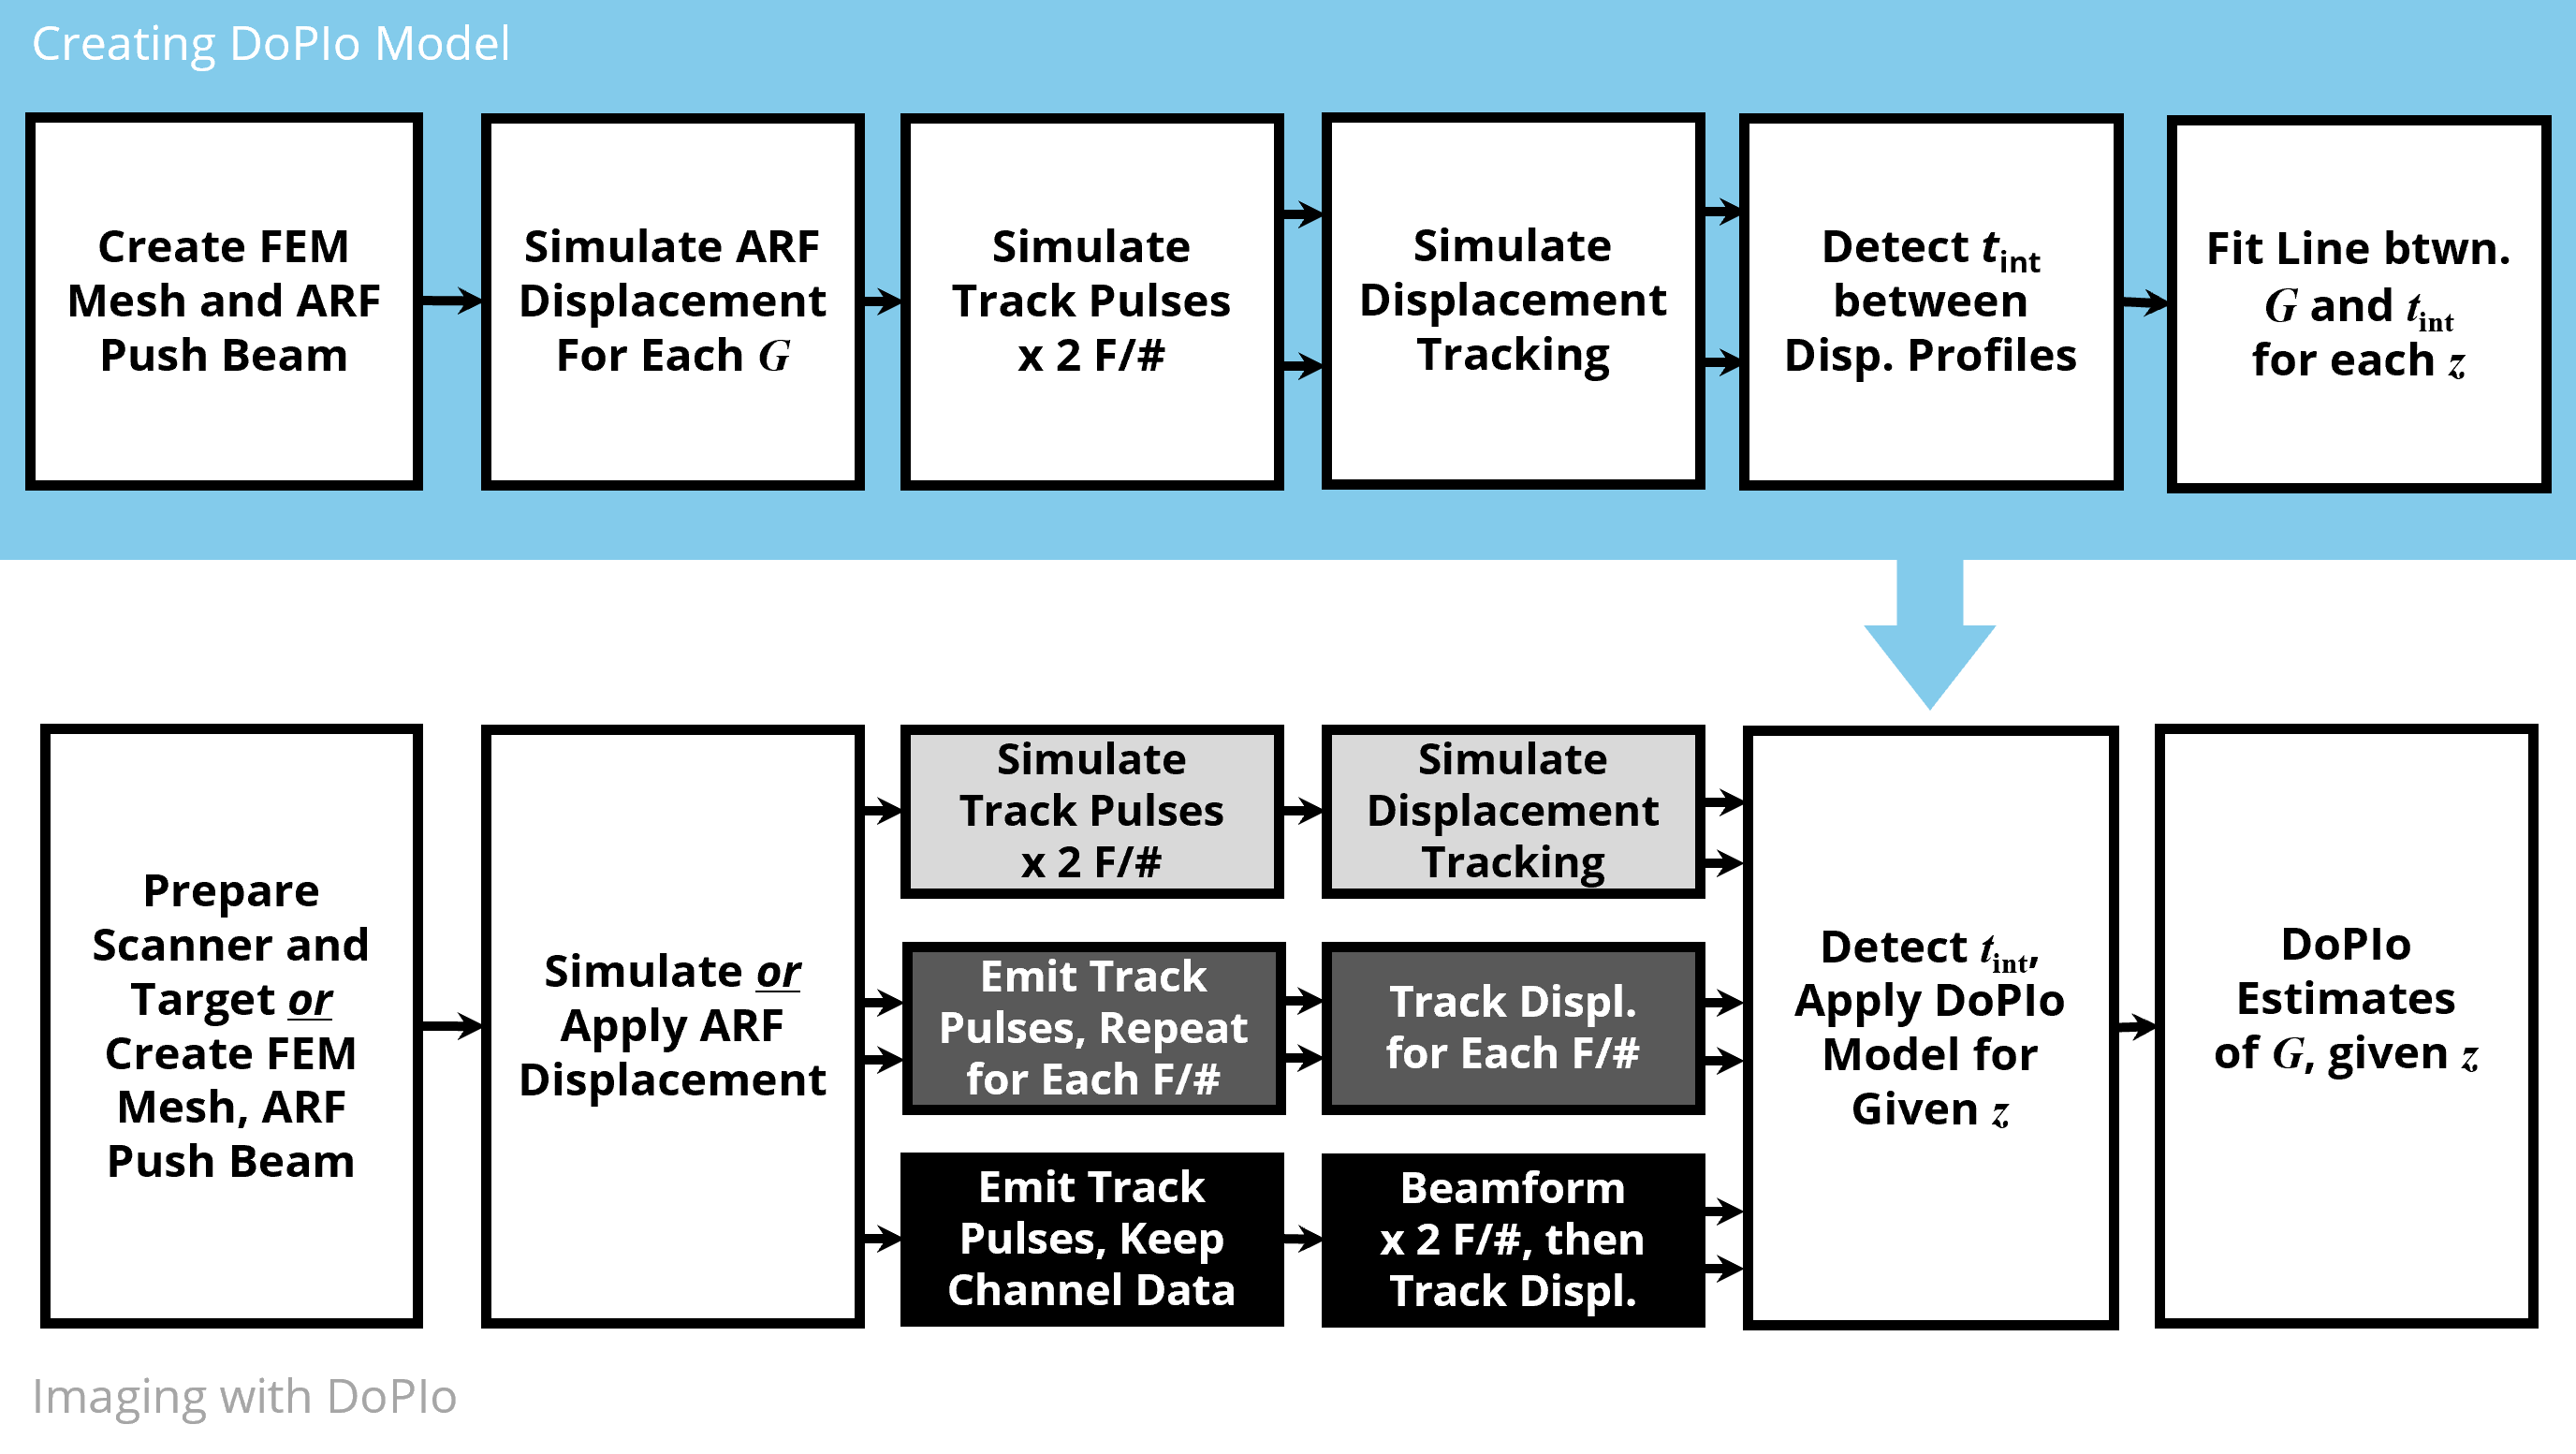
\includegraphics[width=\linewidth]{parts/dopio/fig/workflow.png}
    \caption{
        Flowchart illustrating the DoPIo imaging procedure, including (top row) development of the empirical model and (bottom row) its evaluation using simulated and experimentally acquired displacement datasets. Times-intersect values ($t_{\mathrm{int}}$) are measured at depth $z$ to estimate the shear elastic modulus ($G$).
        }
    \label{fig:flowchart}
\end{figure}

\subsection{Ultrasonic Imaging Simulations}

DoPIo ultrasound was simulated following the procedures originally introduced by Palmeri \emph{et al.}~\cite{palmeri_Experimental_2004,palmeri_Ultrasonic_2006}. Using the linear ultrasound simulator Field-II~\cite{jensen_Calculation_1992,jensen_Field_1997}, ARF excitations were simulated with the specifications of the Philips ATL L7-4 (Bothell, WA, USA), a linear array with an elevational lens focused at 25.0~\si{\milli\meter}. Two ARF focal configurations, F/1.5 and F/3.0, were simulated for comparison, both at a focal depth of 25.0~\si{\milli\meter}. The ARF intensity fields were normalized around the focal depth, scaled to an $I_{\textnormal{SPPA}}$ of 5000~\si{\watt\per\square\centi\meter}, and converted into body forces in the axial direction (i.e. $z$, the direction of acoustic wave propagation) using Eq.~\ref{eq:force}:

\begin{equation}
\vec{F_{z}} = \frac{2 \alpha \vec{I}}{c}
\label{eq:force}
\end{equation}

A sound speed, $c$, of 1540 m/s was assumed, as well as an acoustic attenuation coefficient, $\alpha$, of 0.5 dB/cm/MHz with respect to the transmit frequency. Eq.~\ref{eq:force} was evaluated throughout a hexahedral grid of nodes that were uniformly spaced 0.100 mm apart to represent the ARF push as nodal body forces. This force was applied onto the mesh for 71.2 \si{\micro\second} (300 cycles) at 4.21 MHz, and the resulting displacement response was simulated using the finite element analysis tool LS-DYNA (ANSYS, Canonsburg, PA, USA). Elements were defined as \texttt{*MAT\_ELASTIC} with a density of 1000~\si{\kilo\gram\per\cubic\meter}, Poisson's ratio of 0.499, and Young's moduli based on the experiment described in the following subsections. The outer six elements of the mesh in all directions were replaced with \texttt{*MAT\_PML\_ELASTIC} defined using identical Young's moduli. All non-LS-DYNA operations were performed through MATLAB R2019a (MathWorks Inc., Natick, MA, USA).

Scatterers of normally distributed reflectivity were randomly placed throughout the mesh such that the average scatterer density was 1485~\si{\per\cubic\milli\meter}, corresponding to about 271, 541, and 902 scatterers per resolution cell for F/1.5, F/3.0, and F/5.0 track beams, respectively. Twenty unique realizations of scatterers were simulated. Scatterers were displaced according to the FEM's nodal displacements at every 0.1 ms (i.e. based on a 10 kHz tracking pulse repetition frequency, or PRF), and the displacements were encoded into radio frequency (RF) A-lines using Field-II with two categories of beam sequences. One category involved transmitting a first ARF excitation and tracking it with a narrower tracking beam, then transmitting a second ARF excitation configured as the first and tracking it with a wider tracking beam. We term this sequence a "separate acquisition".  The second category involved transmitting only one ARF excitation and simultaneously tracking it with two tracking beams, one narrower than the other. We term this sequence a "simultaneous acquisition". In the case of the separate acquisition, the tracking beams' focal configuration on transmit matched that on receive. In the case of the simultaneous acquisition, the tracking beam transmit focal configuration matched that of the wider receive focal configuration.

Tracking beam receive focal configurations of F/1.5, F/3.0, and F/5.0 were simulated to support the comparison of DoPIo elastic modulus estimation using the tracking beam pairings (tFc) of F/1.5 and F/3.0 or F/1.5 and F/5.0. These two pairings, each with either separate or simultaneous acquisitions, were combined with either an F/1.5 or F/3.0 ARF excitation, for a total of eight evaluated DoPIo beam sequences (Table~\ref{tbl:fnum}). For all eight beam sequences, tracking beams were two cycles in durations centered at 6.25 MHz. Dynamic receive focusing applied at the center frequency of the track pulses. Using a 10 KHz PRF, ensembles of 6.0 ms were simulated.

% !TeX root = ../../../main.tex


\begin{table*}[bt]
    \centering
    \caption{ARF Push and Track Beam Focal Configuration Combinations (tFc)}
    \begin{tabular}{lll}
    \toprule
    \multicolumn{3}{c}{Wide Track F/3.0} \\ &
      \multicolumn{1}{c}{Sequential Acq.} &
      \multicolumn{1}{c}{Simultaneous Acq.}\\
    \midrule
    \begin{tabular}[c]{@{}l@{}}F/1.5\\ Push\end{tabular} &
      \begin{tabular}[c]{@{}l@{}}Push F/1.5\\ Track Tx F/1.5, Rx F/1.5 and\\ Track Tx F/3.0, Rx F/3.0\end{tabular} &
      \begin{tabular}[c]{@{}l@{}}Push F/1.5\\ Track Tx F/3.0, Rx F/1.5 and\\ Track Tx F/3.0, Rx F/3.0\end{tabular}\\
    \hline
    \begin{tabular}[c]{@{}l@{}}F/3.0\\ Push\end{tabular} &
      \begin{tabular}[c]{@{}l@{}}Push F/3.0\\ Track Tx F/1.5, Rx F/1.5 and\\ Track Tx F/3.0, Rx F/3.0\end{tabular} &
      \begin{tabular}[c]{@{}l@{}}Push F/3.0\\ Track Tx F/3.0, Rx F/1.5 and\\ Track Tx F/3.0, Rx F/3.0\end{tabular}\\
    \bottomrule
    \multicolumn{3}{c}{Wide Track F/5.0} \\ &
      \multicolumn{1}{c}{Sequential Acq.} &
      \multicolumn{1}{c}{Simultaneous Acq.} \\
    \hline
    \begin{tabular}[c]{@{}l@{}}F/1.5\\ Push\end{tabular} &
      \begin{tabular}[c]{@{}l@{}}Push F/1.5\\ Track Tx F/1.5, Rx F/1.5 and\\ Track Tx F/5.0, Rx F/5.0\end{tabular} &
      \begin{tabular}[c]{@{}l@{}}Push F/1.5\\ Track Tx F/5.0, Rx F/1.5 and\\ Track Tx F/5.0, Rx F/5.0\end{tabular}\\
    \hline
    \begin{tabular}[c]{@{}l@{}}F/3.0\\ Push\end{tabular} &
      \begin{tabular}[c]{@{}l@{}}Push F/3.0\\ Track Tx F/1.5, Rx F/1.5 and\\ Track Tx F/5.0, Rx F/5.0\end{tabular} &
      \begin{tabular}[c]{@{}l@{}}Push F/3.0\\ Track Tx F/5.0, Rx F/1.5 and\\ Track Tx F/5.0, Rx F/5.0\end{tabular}\\
    \bottomrule
    \end{tabular}
    \label{tbl:fnum}
\end{table*}


To the generated ensembles, one-dimensional axial displacements were tracked using normalized cross-correlation (NCC) with a 2-wavelength (500 \si{\micro\meter}) tracking kernel and a 0.3-wavelength (80 \si{\micro\meter}) search window~\cite{pinton_Rapid_2006}. A polynomial motion filter was applied to each resulting displacement profile based on the pre-ARF push displacement and the last 2.0 ms of displacement estimates~\cite{giannantonio_Comparison_2011} and upsampled tenfold using piecewise-cubic interpolation~\cite{fritsch_Monotone_1980}. 

\subsection{Empirical Model Development}

To generate a library of $t_{\textnormal{int}}$ for materials of different shear moduli, ten LS-DYNA meshes were created. Elements in each mesh were homogeneously assigned one of 10 shear modulus values ranging from 1 kPa in 4 kPa increments up to 37 kPa. For each mesh, ARF-induced displacement profiles were generated as described above, and then $t_{\textnormal{int}}$ were calculated as the first time the paired tracking beams' displacement profiles intersected after the occurrence of their peak displacements. Times-intersect were measured over an axial range that spanned 10 mm above and below the 25 mm focal depth.

At each axial depth, times-intersect underwent one of two options for nonlinear correlation to shear elastic modulus. The first option was an inverse-square transformation, shown in Equation~\ref{eq:modelinvsq}. This transformation represents a treatment of $t_{\textnormal{int}}$ that resembles shear wave-based techniques, where $G$ is proportional to the inverse square of the time duration of shear wave propagation. 

\begin{equation}
G(t_{\textnormal{int}}, z) = A(z) t_{\textnormal{int}}^{-2} + B(z)
\label{eq:modelinvsq}
\end{equation}

The other option, shown in Equation~\ref{eq:modelarb}, generalizes the relationship in Eq.~\ref{eq:modelinvsq} so that an additional degree of freedom is afforded for the exponent of $t_{\textnormal{int}}$, allowing for a more flexible relationship between it and $G$. Here, $\ln\left(x\right)$ is the natural logarithm of $x$, and $t_{\textnormal{ARF}}$ is the duration of the ARF push.

\begin{equation}
\ln\left( G(t_{\textnormal{int}}, z) \right) = A(z) \ln\left( \frac{t_{\textnormal{int}} - t_{\textnormal{ARF}}}{t_{\textnormal{ARF}}} \right) + B(z) 
\label{eq:modelarb}
\end{equation}

For both models, total least squares linear regression~\cite{markovsky_Overview_2007} was performed between transformed times-intersect and shear moduli. This resulted in a map of polynomial coefficients across different axial positions that could be used to convert time-intersect into a shear modulus estimate for a given set of DoPIo beam parameters.

\subsection{DoPIo Performance Evaluation}

To evaluate the performances of the derived empirical models, additional simulations of ARF displacements were performed using FEM simulations of tissues with different stiffnesses for linearly elastic, isotropic materials with shear moduli from 3 to 27 kPa in 4 kPa increments. The beam sequence and model parameters that led to the smallest median error of shear elastic modulus estimates at the focal depth were considered the best-performing process for DoPIo.

Once the best-performing DoPIo beam sequence and model were identified \emph{in silico}, their accuracy and precision for shear elastic modulus prediction were evaluated \emph{in vitro} in a CIRS Type 049 calibrated elasticity phantom (CIRS, Norfolk, VA, USA). Two-dimensional imaging was achieved by sequentially performing DoPIo data collection in 40 lateral positions spaced 0.48 mm apart, leading to a roughly 2 cm lateral field of view. Each of the four cylindrical inclusions in the phantom were imaged in this manner five separate times on a motion isolation table (ThorLabs, Newton, NJ, USA) using a Verasonics Vantage 256 unit (Kirkland, WA, USA) and the L7-4. The ARF voltage was varied from 35 V to 60 V in 5 V increments to evaluate the impact of ARF magnitude on DoPIo modulus estimates. 

DoPIo performance was similarly evaluated ex vivo in a custom porcine liver-based phantom~\cite{hossain_Viscoelastic_2020}. Here, the liver of a pig sacrificed within 15 hours was acquired from a local butcher. A region of tissue away from fascia and large vasculature was identified, and a prism with 3-cm cross-sectional square sides was excised. A 10 mm diameter cylinder was cut using a disposable biopsy punch (Robbins Instruments, Houston, TX, USA). Then, 600 ml of linearly elastic and acoustically attenuating gelatin-graphite material with an approximate Young's modulus of 15 kPa and attenuation of 0.5 dB/cm/MHz was created~\cite{madsen_Tissue_1978,hall_Phantom_1997}. The excised liver was immersed into the solution such that the gelatin solution filled the punched hole and surrounded the liver. The composite phantom was allowed to solidify for 24 hours in a refrigerator. 

The resulting phantom was returned to room temperature, and then three repeated measures were taken using the L7-4 array in an identical manner to that used to image the CIRS phantom. Since the true elasticity of the liver is unknown and the stiffness of the gelatin mixture is only an approximation, a comparison measurement of shear elasticity was taken using the Siemens Acuson Sequoia clinical scanner (Siemens Healthineers Ultrasound Division, Issaquah, WA, USA). An Acuson 10L4 linear array transducer was placed in the identical position as the L7-4 array, and three 2-D shear wave elasticity images were acquired using its standard clinical SWEI imaging mode. These clinical scanner-acquired shear elasticity estimates were used as the validation stanndard for DoPIo modulus estimates.
